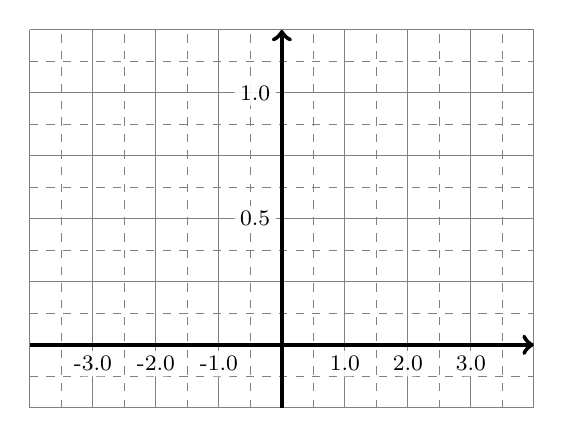
\begin{tikzpicture}[
        every node/.style={
            fill=white,rectangle,inner sep=2pt,
            fill opacity=0.9,text opacity=1,rounded corners=5pt,rounded corners=5pt,
            font=\footnotesize
        },
        scale=0.8
    ]    
% Sets
    \draw[step=0.5,gray,dashed,thin] (-4,-3) grid (4,3);
    \draw[gray] (-4,-3) grid (4,3);
    \draw[->,ultra thick] (-4,-2) -- (4,-2);
    \draw[->,ultra thick] (0,-3) -- (0,3);
% Function
% Labels
    \node[anchor=east,xshift=-2pt] at (0,2) {1.0};
    \node[anchor=east,xshift=-2pt] at (0,0) {0.5};
\foreach\x in {-3.0,-2.0,-1.0,1.0,2.0,3.0}{
    \node[anchor=north,yshift=-2pt] at (\x,-2) {\x};
}
\end{tikzpicture}